\documentclass{beamer} 
\usetheme{Madrid} % My favorite! 
%\usetheme{Boadilla} 
% Pretty neat, soft color. 
%\usetheme{default} 
%\usetheme{Warsaw} 
%\usetheme{Bergen} 
% This template has nagivation on the left 
%\usetheme{Frankfurt} % Similar to the default 
% with an extra region at the top. 
%\usecolortheme{seahorse} % Simple and clean template 
%\usetheme{Darmstadt} % not so good 
% Uncomment the following line if you want 
% % page numbers and using Warsaw theme%
% \setbeamertemplate{footline}[page number] 
%\setbeamercovered{transparent} 
\setbeamercovered{invisible} % To remove the navigation symbols from 
% the bottom of slides
% \setbeamertemplate{navigation symbols}{} 
\usepackage{graphicx} 
%\usepackage{bm} % For typesetting bold math (not \mathbold) 
%\logo{\includegraphics[height=0.6cm]{yourlogo.eps}} % 
\title[Quantised Calculus]{Quantised Calculus in One Variable} 
\author[McDonald, E.]{McDonald, E. S. \\Supervisor: Sukochev, F.} 
\institute[UNSW] { UNSW Australia } 
\titlegraphic{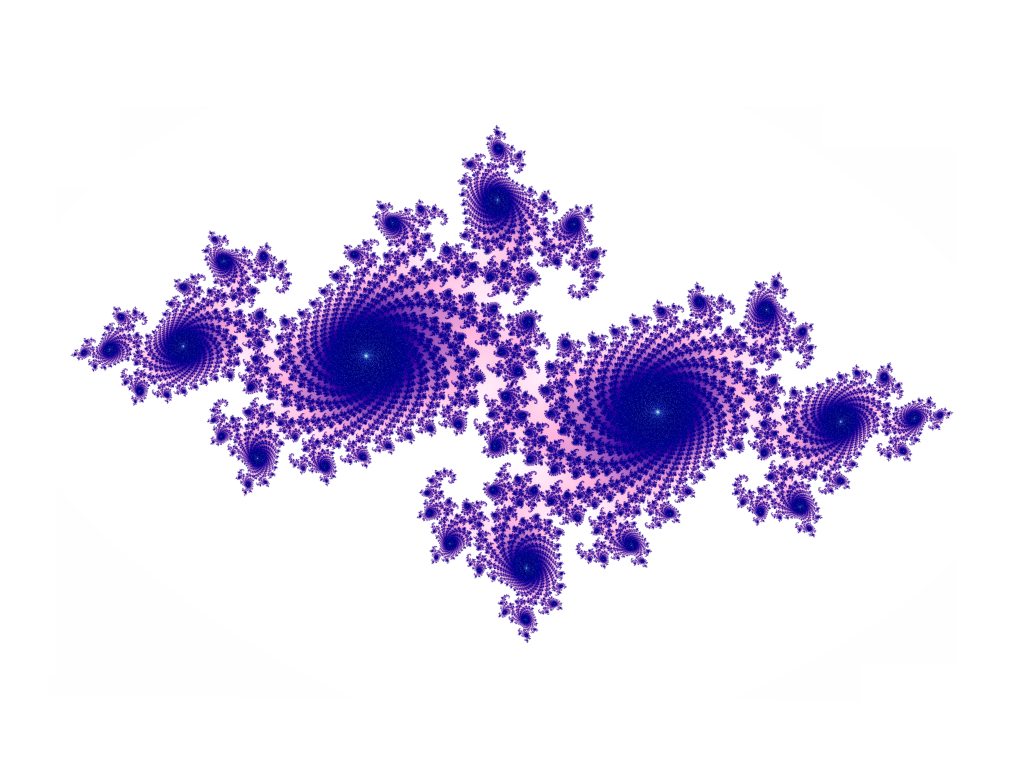
\includegraphics[width=60mm]{Julia_set_(ice).png}}

\date{\today} 


\newcommand{\Rl}{\mathbb{R}}
\newcommand{\Cplx}{\mathbb{C}}
% \today will show current date. 
% Alternatively, you can specify a date. 


\begin{document} 


\begin{frame} 
\titlepage 
\end{frame} % 



\begin{frame} 

\frametitle{Motivation} 

\begin{block}
{Problem:}
What is an infinitesimal?
\end{block}
\begin{block} 
{Problem:}
What is the derivative of a nondifferentiable function?
\end{block}

\end{frame} 

\begin{frame} 
\frametitle{Infinitesimals} 
\begin{itemize}
    \item{} Early calculus (e.g. Leibniz, Newton) made use of infinitesimal quantities:
\end{itemize}
\begin{definition}
    A quantity $x$ is called \emph{infinitesimal} if for any $\varepsilon > 0$,
    \begin{equation*}
        |x| < \varepsilon.
    \end{equation*}
\end{definition}
\begin{definition}
    A quantity $x$ \emph{infinite} if for any $N > 0$, 
    \begin{equation*}
        |x| > N.
    \end{equation*}
\end{definition}
\end{frame} 

\begin{frame} 
\frametitle{Infinitesimals}
This definition was good enough for $18$th century calculus, and many
definitions were formulated in terms of infinitesimals.

For example:
\begin{definition}
    A function $f$ is continuous if $df(x) := f(x+dx)-f(x)$ is infinitesimal
    for any infinitesimal quantity $dx$.
\end{definition}
\begin{definition}
    A function $f$ is differentiable if the quantity
    \begin{equation*}
        f'(x) := \frac{f(x+dx)-f(x)}{dx}
    \end{equation*}
    is not infinite when $dx$ is infinitesimal.
\end{definition}
%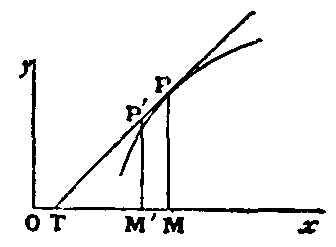
\includegraphics[width=90mm]{Infinitesimal_Calculus_6.png}
\end{frame}

\begin{frame}
\frametitle{Properties of infinitesimals}
\begin{lemma}
    If $x$ is infinitesmal, then $x^{-1}$ is infinite.
\end{lemma} 
\begin{lemma}
    For any $f$,
    \begin{equation*}
        df = \frac{df}{dx}dx
    \end{equation*}
\end{lemma}
\end{frame}

\begin{frame}
\frametitle{Sizes of infinitesimals}
Not all infinitesimals are equal. Intuitively, some should be bigger than others.
Intuitively we expect the following properties:
\begin{itemize}
\item{} If $x > 0$ is infinitesimal, than $x^2 < x$.
\item{} If a function $f$ is smoother than a function $g$, then $df < dg$.
\end{itemize}
\end{frame}

\begin{frame}
\frametitle{Problem}
There is a problem! These definitions make no sense.
\begin{block}
{Problems:}
\begin{itemize}
    \item{} If $x \neq 0$ is infinitesimal, then $|x| < |x|/2$, so $1 < 1/2$.

    \item{} If $x$ is infinite, then $|x| > 2|x|$, so $1 > 2$.
\end{itemize}
\end{block}

So we cannot use the definitions given by $18$th century mathematicians.
\end{frame}
\begin{frame}
    Infinitesimals were rightly banished from mathematics, and the definitions
    of continuity and differentiability were replaced with their modern 
    definitions in terms of limits.
\end{frame}

\begin{frame}
\frametitle{But what \emph{is} an infinitesimal?}
$18$th century mathematicians were still able to use infinitesimals
even though they make no sense. 
\begin{block}
    {Question:}
    Why does calculus using infinitesmals ``work"?
\end{block}
\begin{block}
    {Question:}
    Is there a way to make sense of infinitesimals?
\end{block}
An answer is provided by physics.
\end{frame}

%\begin{frame}
%\frametitle{Quantisation}
%An answer is provided by physics. 
%\begin{block}
%{Classical Mechanics:}
%A physical system is a manifold $\mathcal{M}$. States of the system are points $p \in \mathcal{M}$, 
%and observable quantities are functions $f:\mathcal{M}\rightarrow \Rl$. Quantities evolve
%in time according to the differential equation
%\begin{equation*}
%    \frac{df}{dt} = \{f,H\}
%\end{equation*}
%where $H:\mathcal{M}\rightarrow \Rl$ is a fixed function called the Hamiltonian, and 
%$\{\cdot,\cdot\}$ is the \emph{Poisson bracket}, a differential operator defined
%by the geometry of the manifold.
%\end{block}

%\end{frame}

%\begin{frame}

%\begin{block}
%{Quantum Mechanics:}
%A physical system is a Hilbert space $\mathcal{H}$. States of the system are vectors $\psi \in \mathcal{H}$, 
%and observable quantities are linear operators $O:\mathcal{H}\rightarrow\mathcal{H}$. Quantities evolve
%in time according to the differential equation
%\begin{equation*}
%    \frac{dO}{dt} = \frac{i}{\hbar}[O,H]
%\end{equation*}
%where $H:\mathcal{H}\rightarrow\mathcal{H}$ is a fixed operator called the Hamiltonian, and
%$[\cdot,\cdot]$ is the \emph{commutator}, given by $[O,H] = OH-HO$.
%\end{block}
%\end{frame}

\begin{frame}
\frametitle{Physics}
        \begin{columns}[T]
            \begin{column}{.5\textwidth}
                \begin{block}{Classical Mechanics}
                    \begin{itemize}
                        \item{} State space is a manifold $\mathcal{M}$
                        \item{} States are points $p \in \mathcal{M}$
                        \item{} Quantities are functions $f:\mathcal{M}\rightarrow\Cplx$.
                        \item{} Quantities evolve according to
                        \begin{equation*}
                            \frac{df}{dt} = \{f,H\}
                        \end{equation*}
                    \end{itemize}
                \end{block}
            \end{column}
        
        
            \begin{column}{.5\textwidth}
                \begin{block}{Quantum Mechanics}
                    \begin{itemize}
                        \item{} State space is a Hilbert space $\mathcal{H}$
                        \item{} States are vectors $\psi \in \mathcal{H}$
                        \item{} Quantities are operators $O:\mathcal{H}\rightarrow\mathcal{H}$
                        \item{} Quantities evolve according to
                        \begin{equation*}
                            \frac{dO}{dt} = \frac{i}{\hbar}[O,H]
                        \end{equation*}
                    \end{itemize}
                \end{block}
            \end{column}
        \end{columns}
\end{frame}

\begin{frame}
\frametitle{Quantisation}
\begin{itemize}
\item{} Quantisation is the process of converting a classical mechanical system to a quantum mechanical system
\item{} In general, doing this in a satisfying way is an unresolved problem.
\end{itemize}
\end{frame}

\begin{frame}
\frametitle{Quantisation}
Quantisation should look like this:
\begin{itemize}
    \item{} Manifolds should be replaced with Hilbert spaces (e.g, replace $\mathcal{M}$ with $L^2(\mathcal{M})$)
    \item{} Functions $f:\mathcal{M}\rightarrow \Cplx$ should be replaced with operators (e.g. replace $f$ with $M_f$)
\end{itemize}
\end{frame}

\begin{frame}
\frametitle{Quantising calculus}
\begin{itemize}
\item{} The setting for calculus (in one variable) is a manifold, $\Rl$.
\item{} The objects of study in calculus are functions $f:\Rl\rightarrow\Cplx$.
\end{itemize}
This is like ``classical" physics. Can we find a ``quantum" counterpart?
\end{frame}

\begin{frame}
\frametitle{Quantising calculus}
\begin{itemize}
\item{} Instead of $\Rl$, we should talk about $L^2(\Rl)$
\item{} Instead of functions on $\Rl$, we should talk about operators on $L^2(\Rl)$. 
\end{itemize}
This includes ordinary calculus, since any $f:\Rl\rightarrow\Cplx$
can be encoded as a pointwise multiplication operator $M_f$.
\end{frame}

\begin{frame}
\frametitle{Quantising calculus}
Our class of objects of study is therefore massively expanded.
        \begin{columns}[T]
            \begin{column}{.5\textwidth}
                \begin{block}{Classical Calculus}
                    \begin{itemize}
                        \item{} $\Rl$
                        \item{} Complex valued function
                        \item{} Real valued function                       
                        \item{} Range of a function
                    \end{itemize}
                \end{block}
            \end{column}
        
        
            \begin{column}{.5\textwidth}
                \begin{block}{Quantised Calculus}
                    \begin{itemize}
                        \item{} $L^2(\Rl)$
                        \item{} Operator $F:L^2(\Rl)\rightarrow L^2(\Rl)$
                        \item{} Self adjoint operator
                        \item{} Spectrum of an operator
                    \end{itemize}
                \end{block}
            \end{column}
        \end{columns}
        
\end{frame}

\begin{frame}
\begin{block}
{Question:}
    We now have many more objects to consider in calculus. 
    Do we have something like infinitesimals?
\end{block}
\end{frame}

\begin{frame}
\frametitle{Compact operators}
\begin{definition}
    An operator $T$ on a Hilbert space $\mathcal{H}$
    is called \emph{compact} if for any $\varepsilon > 0$
    there is a finite dimensional subspace $E$ such that 
    \begin{equation*}
        \| T|_{E^\perp}\| < \varepsilon
    \end{equation*}
\end{definition}
This is very much like the $18$th century definition of infinitesimal!
A compact operator is ``infinitesimal modulo finite dimensional subspaces".
\end{frame}

\begin{frame}
    So we have something in quantised calculus that looks
    like an $18$th century
    infinitesimal. How much of the classical use of infinitesimals
    can we recover?
\end{frame}

\begin{frame}
\frametitle{Compact operators}
\begin{block}
    {Question:}
    How can we measure the size of a compact operator?
\end{block}
The answer should be analogous to the ``size" of an infinitesimal.
\end{frame}

\begin{frame}
\frametitle{Compact operators}
If $T$ is a compact operator, we define
\begin{definition}
The $n$th singular value of $T$ is
\begin{equation*}
    \mu_n(T) := \inf\{\|T-R\|\;:\;\operatorname{rank}(R) \leq n\}.
\end{equation*}
\end{definition}
The sequence $\{\mu_n(T)\}_{n=1}^\infty$ is a decreasing sequence of 
real numbers approacing $0$.
\end{frame}

\begin{frame}
\begin{block}
{Idea:}
We can quantify the size of $T$ by the rate of decay of $\{\mu_n(T)\}_{n=1}^\infty$.
\end{block}
Does this correspond to the $18$th century notions of the size of an infinitesimal?
\end{frame}

\begin{frame}
\frametitle{Submultiplicativity}
\begin{theorem}
    If $T$ and $S$ are compact operators, then
    \begin{equation*}
        \mu_n(TS) \leq \mu_n(T)\mu_n(S)
    \end{equation*}
\end{theorem}
So if $T$ is infinitesimal (i.e. compact), then ``$T^2 < T$" (in this sense).
\end{frame}

\begin{frame}
\frametitle{Quantised differential}
\begin{definition}
    If $f:\Rl\rightarrow\Cplx$, then the \emph{operator}
    $df$ is defined as
    \begin{equation*}
        df(g)(x) = \lim_{\varepsilon\rightarrow 0}\int_{\Rl\setminus (x-\varepsilon,x+\varepsilon)} \frac{f(x)-f(t)}{x-t}g(t)\;dt.
    \end{equation*}
    for $g \in L^2(\Rl)$.
\end{definition}
\end{frame}

\begin{frame}
\frametitle{Smoothness and differentials}
This is the topic of my thesis.
\begin{block}
    {Question:}
    What is the relationship between the smoothness of $f$
    and the size of $df$?    
\end{block}
\end{frame}

\begin{frame}
\frametitle{Smoothness and differentials}
There are some initial results:
\begin{itemize}
    \item{} $df$ is of finite rank if and only if $f$ is rational.
    \item{} If $f$ is continuous, then $df$ is compact.
\end{itemize}
This is exactly what we wanted. Can we do better?
\end{frame}

\begin{frame}
\frametitle{More advanced results}
\begin{itemize}
    \item{} $df$ is compact if and only if $f$ has vanishing mean oscillation.
    \item{} $df$ is bounded if and only if $f$ has bounded mean oscillation.
\end{itemize}
\end{frame}

\begin{frame}
\frametitle{Schatten-Von Neumann Classes}
\begin{definition}
    The set $\mathcal{S}_p$ is the set of compact operators such that
    \begin{equation*}
        \{\mu_n(T)\}_{n=1}^\infty \in \ell^p.
    \end{equation*}
\end{definition}
\end{frame}

\begin{frame}
\frametitle{Schatten-Von Neumann Classes}
The following is due to V.V. Peller (1984)
\begin{theorem}
    $df \in S_p$ if and only if $f \in B_{pp}^{1/p}$.
\end{theorem}
$B_{pp}^{1/p}$ is a Besov space.
\end{frame}

\begin{frame}
    Can we do better?
\end{frame}

\begin{frame}
\frametitle{Schatten-Lorentz classes}
The Schatten-Lorentz class $\ell^{p,q}$, for $p \in (0,\infty)$ and $q \in (0,\infty]$ is defined as
\begin{definition}
    A sequence $\{x_n\}_{n=0}^\infty$ is $\ell^{p,q}$ if
    \begin{equation*}
        \sum_{n=0}^\infty x_n^q (1+n)^{q/p-1} < \infty
    \end{equation*}
    for $q < \infty$
    and
    \begin{equation*}
        \sup_{n\geq 0}\; (1+n)^{1/p}x_n < \infty.
    \end{equation*}
\end{definition}
\end{frame}
\begin{frame}
\frametitle{}
\begin{definition}
The Schatten-Lorentz class $S_{p,q}$ is the set
of compact operators $T$ such that $\{\mu_n(T)\}_{n=1}^\infty \in \ell^{p,q}$.
\end{definition}
For what functions $f$ is in $df \in S_{p,q}$.
\end{frame} 

\end{document}